\section{ADC}
ADC eller A/D converter er en enhed der benyttes til at omdanne et elektrisk analog signal til et digitalt signal som kan viderebearbejdes i software. 
Den ADC som sidder på PIC32mx250f128b\fxnote{kilde} er en 10 bit ADC, som kan have op til 9 analoge inputs. På UCN boardet er 6 mulige inpits hvoraf gruppen kun anvender 3 til lyssensorerne. 

\begin{figure}[h!]
  \centering
  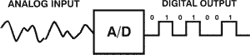
\includegraphics[width=0.7\textwidth]{figures/A_D_converter.png}
  \caption{ADC diagram.\cite{ADC_figur}}
  \label{adcDiagram}
\end{figure} 
\fxnote{fix figur og kilde}
%kilde til http://www.microchip.com/wwwproducts/en/PIC32MX250F128B(hashtag)documents
Den anvendte ADC er implementeret ved hjælp af "ADC reference manual" fra microchip, som er et generekt datablad for nogle af PIC32 processorene. Her er de nødvendige opsætninger som skal foretages for at anvende ADC'en efter den ønskede hensigt.
\newline



ADC'en er implementeret ved hjælp af fremgangsmåden anvist i databladet. Her sættes en række registre op efter den ønskede opsætning. 

\begin{figure}[h!]
  \centering
  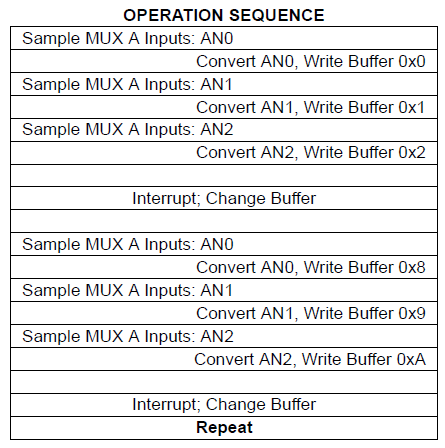
\includegraphics[width=0.7\textwidth]{figures/operation_sequence.png}
  \caption{Operations sekvens.}\fxnote{kilde til datablad, evt lav flow chart istedet for denne figur}
  \label{handlingsekvens}
\end{figure} 

Den angivne sekvens angivet på figur \ref{handlingsekvens}, angiver hvorledes ADC'en operere. 

En ADC kan generer noget kaldet "Aliasing" som er kopier af signalet, som bliver genereret ved samplings frekvensen. Dette filtreres væk vha. et low-pass filter.